\documentclass{llncs}
\usepackage{graphicx}
\usepackage{placeins}
%
\begin{document}
\pagestyle{headings} 
\mainmatter
%
\title{2D Optimal Packing with Population Based Algorithms}
%
\author{Desislava Koleva\inst{1}, Maria Barova\inst{2}, Petar Tomov\inst{2}}
%
\authorrunning{Desislava Koleva} 
%
\tocauthor{Desislava Koleva, Maria Barova, Petar Tomov}
%
\institute{University College London, Department of Computer Science, Gower Street, London, WC1E 6BT, United Kingdom\\
\email{desislava.koleva.15@ucl.ac.uk}
\and
Institute of Information and Communication Technologies, Bulgarian Academy of Sciences, acad. G. Bonchev Str, Block 2, 1113 Sofia, Bulgaria}
%
%Desislava Koleva desislava.koleva.15@ucl.ac.uk
%Maria Barova m.barova@iit.bas.bg
%Petar Tomov p.tomov@iit.bas.bg 
%
\maketitle
%
\begin{abstract}
This study addresses application of population based optimization heuristics to the solution of packing problems as part of optimal cutting tasks in the field of operations research. Such problems are very common in the industrial material cutting. The problem has one, two or three dimensional variations. The focus of this paper is the two dimensional case of steel sheet cutting. A description of two dimensional plates is supplied as input for the algorithm. The output is in the form of coordinates of the plates in the steel sheet and angle of rotation for each plate. Population based global optimization heuristics are used for optimal packing. All experiments are done with open source libraries for 2D geometry and population based heuristics. 
\keywords{Optimal Cutting Problem, Optimal Packing, Evolutionary Algorithms, Optimization}
\end{abstract}
%
\section{Introduction}
%
Optimal packing problem is an optimization problem in mathematics that involves attempting to pack objects together into one or many containers. A tipical goal is to fill a single container as densely as possible. This problem is related to real life packaging (in fact optimal cutting) problem as described in [1,2]. This study is related to the problem presented at ESGI120 [2] and ESGI113 [3]. The goal is to cut optimally into pieces a sheet of steel without overlapping them. The cutting result shapes are irregular not self-intersecting polygons. The problem presented at ESGI113 was less complicated than the problem presented at ESGI120, because both the peaces and the sheet were of rectangular shape. A similar problem is well presented in [4]. With irregular shapes and when the angle of orientation of the given shape is unconstrained, the general nesting approaches are not particularly successful [5]. 

This section starts with description of the problem and refers to related work in a brief review. Section 2 points out the geometric considerations necessary to understand this work. Section 3 describes the underlying rules and criteria used to build the GA based heuristic approach, which is proposed in the same section. Section 4 describes the evaluation of the proposed approach and presents some of the obtained results. Finally, the last section draws conclusions and includes some comments about future work.
%
\subsection{Problem description}
%
The placement of shapes can be found in literature under the keywords of "optimal packing". When packing on a limited stock sheet, the
goal is to maximize the percentage of stock sheet utilization, which is equivalent to maximizing the number of shapes placed inside the plate. The problem proposed to be solved does not considerer orientation constraints, so, any rotation of the given shape can be allowed. When stock sheet borders need to be taken into account, the orientation of the shapes may be extremely important as it will be shown in the experimental part of this study.

In this work, we propose to solve the problem of Packing of Irregular Shapes (PIS) on a limited stock sheet (a rectangle) by heuristic methods.
%
\subsection{Related work}
%
There are references in the literature to the Packing Problem since the 10th century. Persia, Abul Wefa produced a square dissection problem which often reappears today. Henry Ernest Dudeney's dissection puzzles were famous in the early part of last century, and in three dimensions Piet Hein's Soma Cube (Van Delft and Botermans, 1978) in which pieces have not only have to be packed into a cube, but must also be sufficiently stable to balance on a central point, is perhaps the most interesting packing problem to date [6]. However it is only recently that industrial packing problems have been approached from a scientific viewpoint. It should be noted that the rectangular packing problem is known to be NP-complete and therefore it is often not possible to provide exact solutions within a reasonable time limit. Practical problems are not restricted to those involving rectangles, but because of the increased complexity of non-rectangular problems a large proportion of the published work to date has been limited to the packing of rectangles or cuboids [6]. 
%
\subsection{Genetic Algorithms}
%
Genetic algorithms (GAs) are search heuristic inspired by the process of natural selection [7,8]. GAs are routinely used to generate points (candidate solutions) into solutions space. By application of techniques for inheritance (crossover), mutation and selection generated points can get closer to the optimums. GAs are classified also as population based algorithms, because each point into solution space represents an individual inside GAs population. Each individual has a set of properties which are subject of mutation and modification (usually crossover). Traditional representation of the properties is a binary sequence of 0s and 1s, but other encodings are also possible (binary tree for example) [9].

Optimization usually starts from random generated population of individuals, but this is also subject of implementation. The optimization process is iterative and the population in each iteration is called generation. For each individual of the generation fitness value is calculated. Fitness value usually represents the objective function which is a subject of optimization. The most fit individuals into the population are selected (according selection rule) and recombined (crossover and/or mutation) to form a new generation. This new generation is used in the next iteration of the algorithm. Algorithm termination is usually achieved by reaching maximum number of generations or by reaching the desired level of the fitness value [9].

In order to run GAs it is necessary to provide: 1. Genetic representation of the solution space (solution domain); 2 an appropriate fitness function to evaluate the solution domain. Once these two conditions are met GAs can proceed with population initialization and iterative population improvement by repetitive application of selection, crossover, mutation and individuals’ evaluation [9].
%
\section{Geometric considerations}
%
All shapes are represented as polygons. Arcs are approximated with small lines. Holes inside the shapes are not considered by definition [2]. Each polygon is represented as set of vertices [10]. It is not allowed the polygons to overlap. All polygons must be entirely placed inside the stock sheet. To guarantee that two polygons do not overlap and are positioned as close as possible, a concept similar to no-fit-polygon (NFP) is used. The first polygon is positioned on the plane and is considered as the fixed piece. The second polygon is tracing sheet the edge of the fixed polygon. To ensure that any shape is entirely placed inside the stock sheet, a concept similar to inner-fit-polygon (IFP) is used. The IFP is the geometric place of all the points where the reference point of the piece to place can be positioned, so that the piece can be completely placed inside the stock sheet [5]. The computation of NFPs is a very time consuming operation for nonconvex polygons. As a new NFP needs to be recomputed whenever a new relative orientation between two polygons is considered, the complexity of this operation must be taken into account when developing heuristics.

The objective of the PIS problem is to place the largest number of irregular shapes inside a limited rectangular stock sheet, where all the shapes have different orientation. In its most general formulation, there are no constraints on the selection of the shapes orientation used to build the layout and different orientations should be tested in order to find the one that takes the most out of the stock sheet’s borders.

To build a layout for the PIS problem, it is necessary to define some parameters:

* the orientation of each shape, i.e. the rotation angle relative to the original orientation;

* the placement point of each shape positioned;

* the order in which shapes are placed on the sheet;

One of the problems arising in all types of nesting problems is the intrinsic difficulty to deal with geometry, as usually shapes are not regular and not even convex. Besides this difficulty, the necessity of considering all the non-overlapping constraints naturally leads to the consideration of heuristic procedures [5]. 
%
\section{Genetic Algorithm for Optimal Packing Order}
%
Reading of the input data is done from a text file with listed coordinates of the polygons. During GA's population initialization, different individuals are initialized either with all plates oriented horizontally, vertically or in random angle of rotation. This way a better population diversity is achieved. Eight different plate orderings are applied to GA's individuals: unchained input order, randomly shuffled, sorted by plates width, sorted by plates height and bounding rectangle [10]. The initial population is than evaluated by packing with the length of the bounding rectangles. 

As GA selection rule parent individuals are randomly chosen. For plates ordering in the GA's individuals permutation crossover is applied. The resulting child is kept on the place of the worst individual in the population (indirect elitism rule). Mutation is applied over the newly created individual in the form of rotation in a small random angle and change in the order of two randomly selected plates. For newly created individual to be evaluated, a procedure for plates' packing is applied. The individual fitness value is the length of the steel sheet used after packing is applied. 

\vspace{4 mm}
The basic algorithm is as follows:

\vspace{4 mm}
1. Load plates information and store them as polygon objects;

2. Initialize random GA population;

3. Optimization:

\hspace{4 mm} 3.1 Select parents;

\hspace{4 mm} 3.2 Crossover;

\hspace{4 mm} 3.3 Mutation;

\hspace{4 mm} 3.4 Pack polygons;

\hspace{4 mm} 3.5 Measure used sheet length as fitness value;

\hspace{4 mm} 3.6 Keep newly generated chromosome;

\hspace{4 mm} 3.7 Stop if predefined number of generations is reached;

\hspace{4 mm} 3.8 Repeat from 3.1;%
\section{Experiments and Results}
%
All experiments are done with open source software [10] developed by the authors with the support of Velbazhd Software LLC. The software solution is using Java AWT and JST library polygon functionality. Custom implementation of GA is proposed and capabilities for Apache GA Framework usage are provided. GA is applied with the parameters listed in Tab. 1.
%
\begin{table}[]
\centering
\label{tab1}
\begin{tabular}{@{}ll@{}}
\multicolumn{1}{c}{{ \textbf{Parameter}}} & \multicolumn{1}{c}{{\textbf{Value}}} \\
\multicolumn{1}{|l|}{generation gap}                                                  & \multicolumn{1}{l|}{0.98}                                                         \\
\multicolumn{1}{|l|}{crossover rate}                                                  & \multicolumn{1}{l|}{0.90}                                                         \\
\multicolumn{1}{|l|}{mutation rate}                                                   & \multicolumn{1}{l|}{0.01}                                                         \\
\multicolumn{1}{|l|}{maximum generations}                                             & \multicolumn{1}{l|}{100}                                                         \\
\multicolumn{1}{|l|}{number of individuals}                                           & \multicolumn{1}{l|}{137}                                                           \\
\multicolumn{1}{|l|}{number of variables}                                             & \multicolumn{1}{l|}{318}                                                     \\
\multicolumn{1}{|l|}{inserted rate}                                                                       & \multicolumn{1}{l|}{100 \%}                                                                            \\
\end{tabular}
\vspace{2 mm}
\caption{Genetic algorithm parameters.}
\end{table}
\FloatBarrier
%
Three independent experiments were executed (Fig. 1, Fig. 2 and Fig.3) with the same input data. The input data are taken from ESGI 120 case study [2], as real industrial task presented by STOBET Ltd. 
%
\begin{figure}
	\centering
	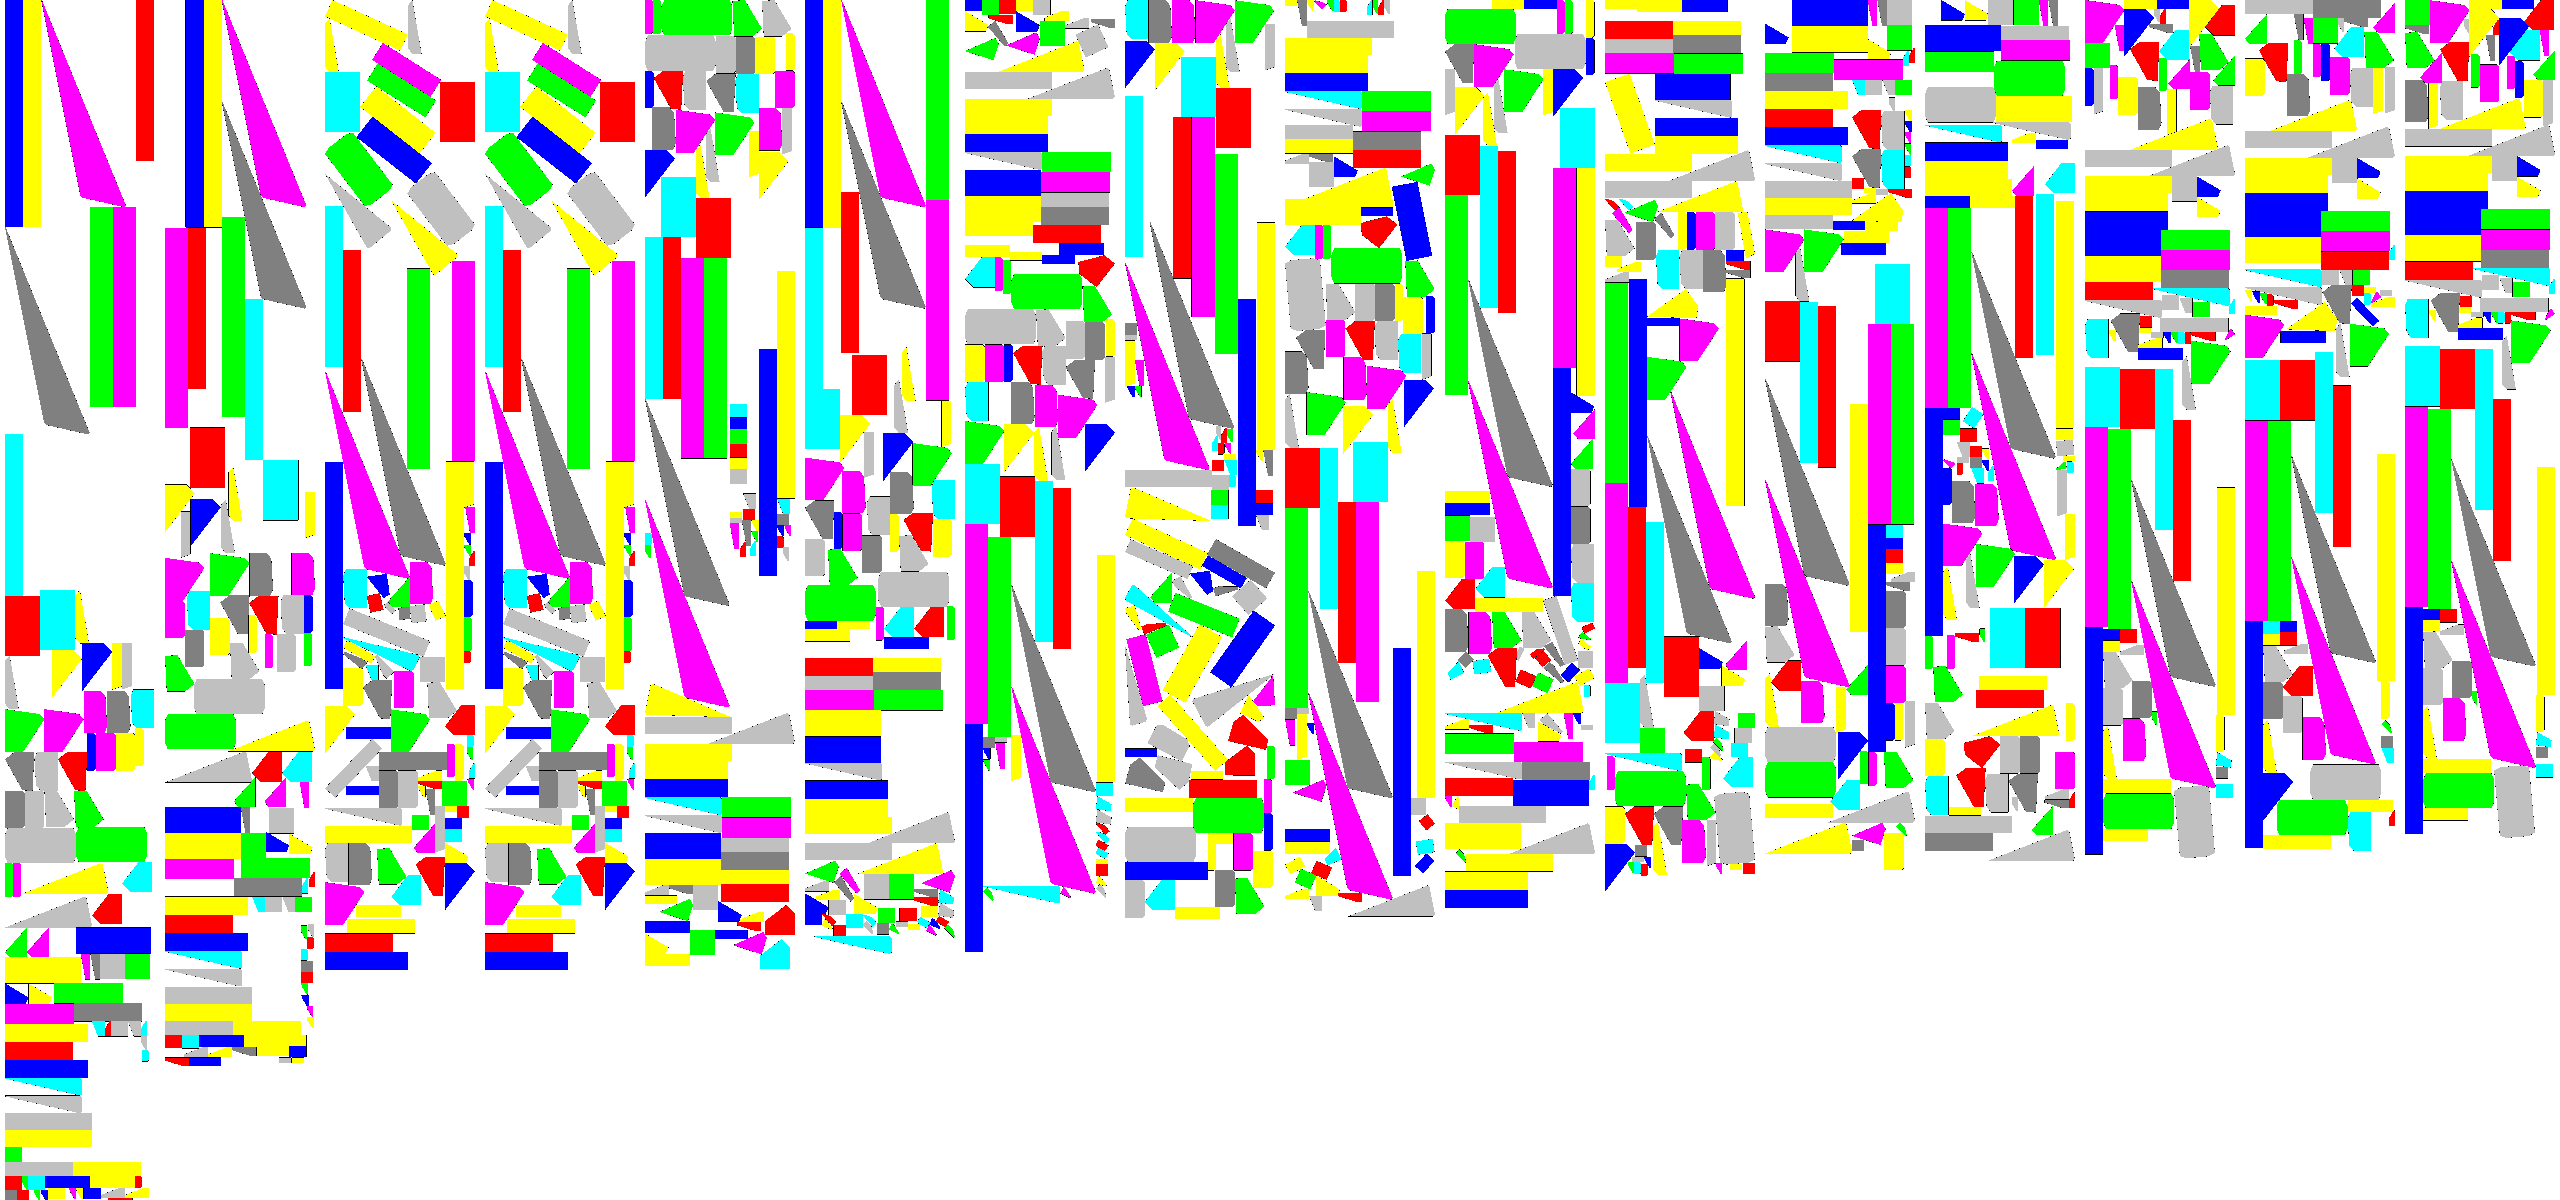
\includegraphics[width=12.62cm,height=7.88cm]{fig01.png}
	\caption{Experiment 1 - final packing solution.}
	\label{fig:Graph}
\end{figure}
%
\begin{figure}
	\centering
	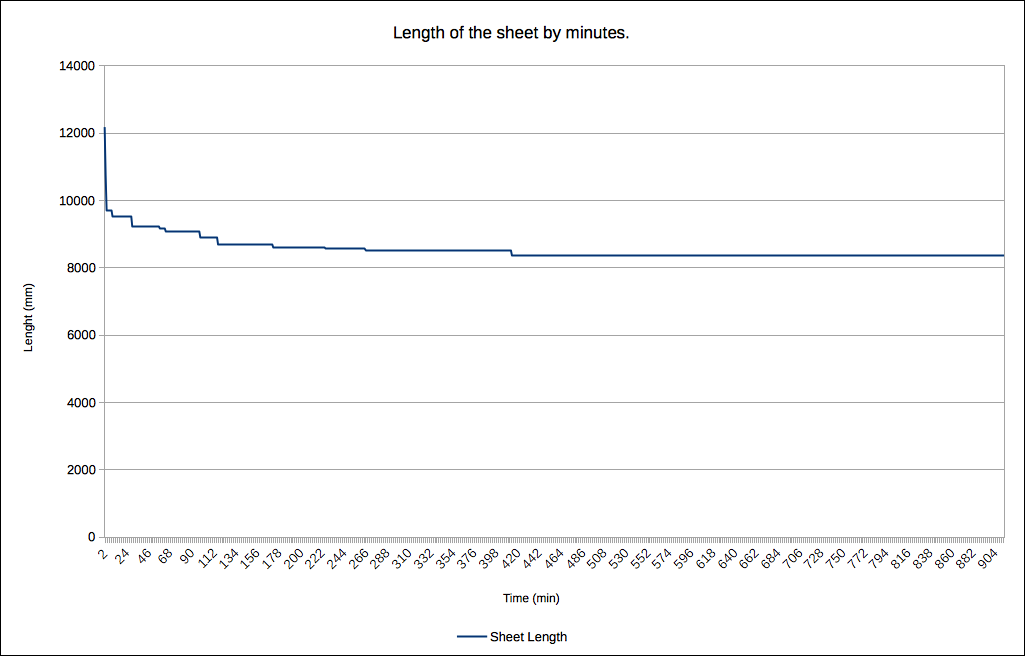
\includegraphics[width=12.62cm,height=7.88cm]{fig02.png}
	\caption{Experiment 2 - final packing solution.}
	\label{fig:Graph}
\end{figure}
%
\begin{figure}
	\centering
	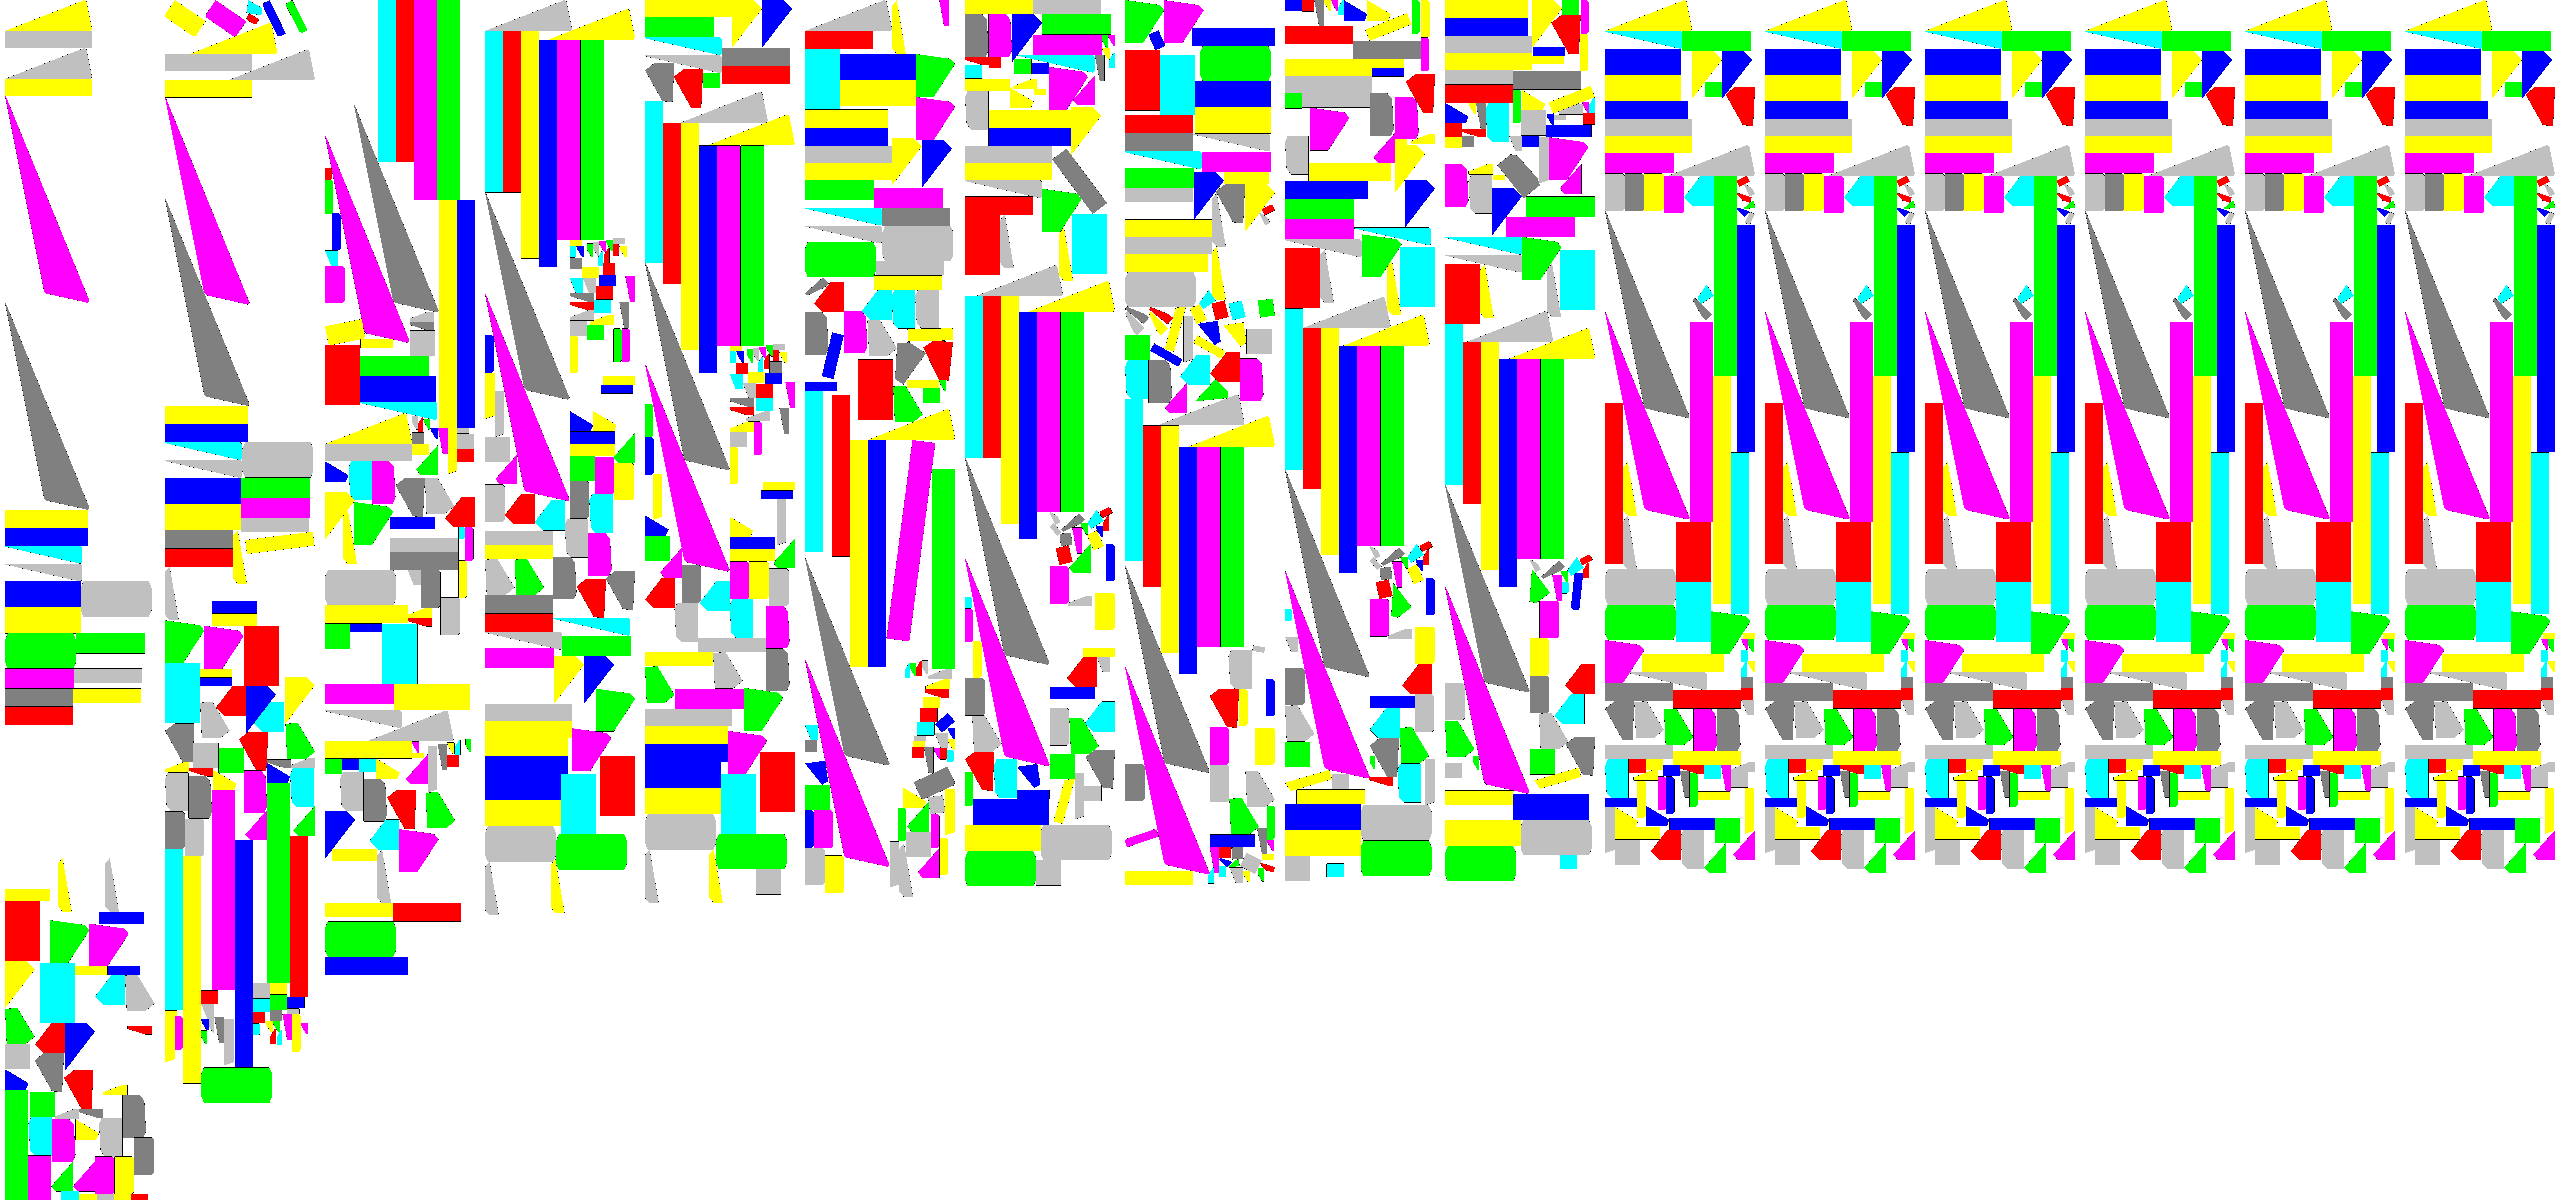
\includegraphics[width=12.62cm,height=7.88cm]{fig03.png}
	\caption{Experiment 3 - final packing solution.}
	\label{fig:Graph}
\end{figure}
\FloatBarrier

The convergence of the experiments is similar as it is shown on Fig. 4. Convergence is stairs like because GA is working on a discrete basis and elitism rule was applied.

\begin{figure}
	\centering
	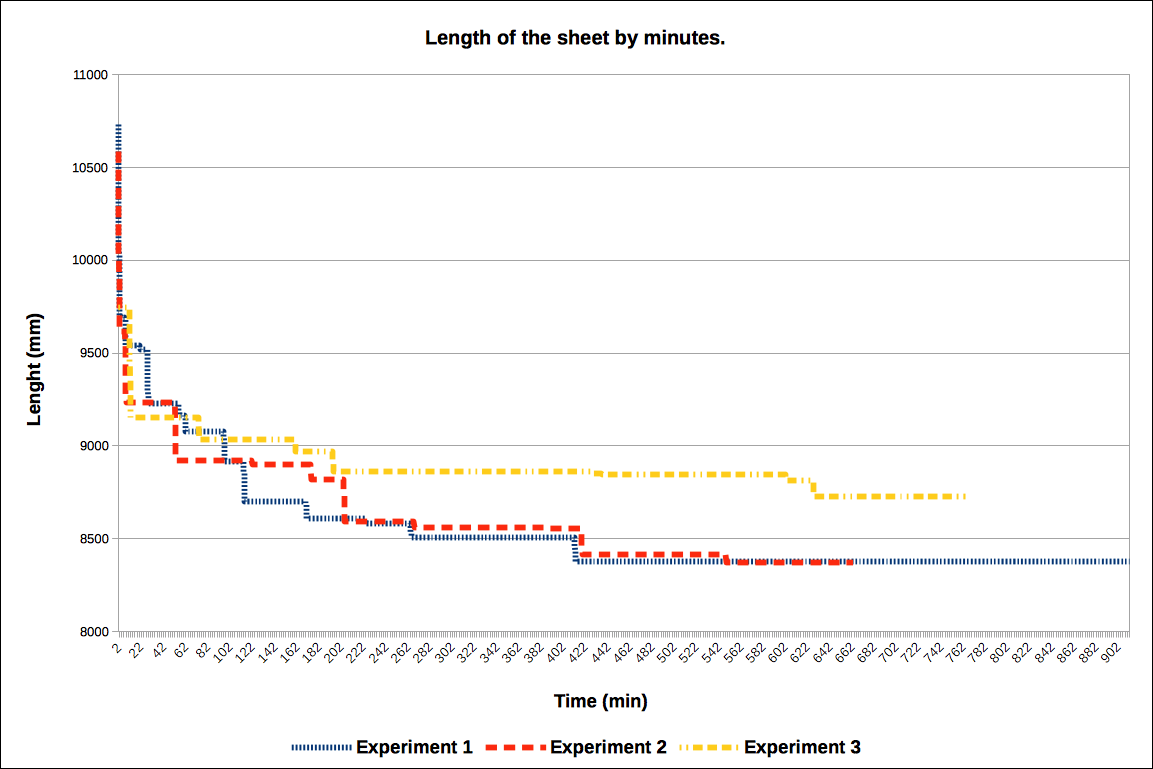
\includegraphics[width=12.62cm,height=7.88cm]{fig05.png}
	\caption{Optimization convergence comparison. On the Y-axis the length of the used steel sheet is presented. On the X-axis optimization time is presented (in minutes) on an average performing laptop.}
	\label{fig:Graph}
\end{figure}
\FloatBarrier
%
It is obvious that the two biggest triangles are problematic in the optimal packing and GA is not very capable to deal with this local optima problem.
%
\section{Conclusions}
%
Usage of GAs for PIS is a promising approach, but solutions are suboptimal and relatively near to the global optimum. In real industrial application GA may be combined with interactive human assistance in order to achieve faster and better solutions. Much greater improvment of the algorithm can be achieved if it is implemented as a distributed computing solution as it is described in [11, 12, 13]. 
%
\section*{Acknowledgements}
%
%
This work was supported by private funding of Velbazhd Software LLC.
%
% ---- Bibliography ----
%
\begin{thebibliography}{}
%
\bibitem[1]{evti:fid}
Evtimov, G., Fidanova, S.:
Ant Colony optimization algorithm for 1D Cutting Stock Problem.
Proceedings of 11th Annual Meeting of the Bulgarian Section of SIAM, FASTUMPRINT, Sofia, Bulgaria, 24--25 (2016)
%
\bibitem[2]{evti}
Evtimov, G.:
Project 2: Optimal cutting problem.
STOBET Ltd., 120th European Study Group with Industry, Sofia, Bulgaria  (2016)
%
\bibitem[3]{avdz:bal}
Avdzhieva, A., Balabanov, T., Evtimov, G., Kirova, D., Kostadinov, H., Tsachev, Ts., Zhelezova, S., Zlateva N.:
Optimal Cutting Problem.
Problems \& final reporst of 113-th European Study Group with Industry, FASTUMPRINT, Sofia, Bulgaria, 49--61 (2015)
%
\bibitem[4]{mart:mon}
Martelloa, S., Monacib, M.:
Models and algorithms for packing rectangles into the smallest square.
Computers \& Operations Research, vol. 63, 161--171 (2015)
%
\bibitem[5]{tere:mig}
Teresa Costa, M.,  Miguel Gomes, A., Oliveira, J.:
Heuristic approaches to large-scale periodic packing of irregular shapes on a rectangular sheet.
European Journal of Operational Research, vol. 192, 29--40 (2009)
%
\bibitem[6]{dows:dows}
Dowsland, K., Dowsland, W.:
Packing problems.
European Journal of Operational Research, vol. 56, 2--14 (1992)
%
\bibitem[7]{eibe}
Eiben, A. E:
Genetic algorithms with multi-parent recombination,
PPSN III: Proceedings of the International Conference on Evolutionary Computation. The Third Conference on Parallel Problem Solving from Nature: 78–87. ISBN 3-540-58484-6, (1994)
%
\bibitem[8]{ting}
Ting, Chuan-Kang:
On the Mean Convergence Time of Multi-parent Genetic Algorithms Without Selection. Advances in Artificial Life: 403–412. ISBN 978-3-540-28848-0, (2005)
%
\bibitem[9]{bala:znak}
Balabanov T., Zankinski I., Shumanov B.:
Slot Machines RTP Optimization with Genetic Algorithms,
8th International Conference, NMA 2014, Borovets, Bulgaria, Numerical Methods and Applications Lecture Notes in Computer Science, vol. 8962, 55--61 (2015)
%
\bibitem[10]{bal:evti}
Balabanov, T., Evtimov, G., Koleva, D.:
ESGI 120 - Problem 2 - Genetic Algorithm Solver.
https://github.com/VelbazhdSoftwareLLC/ESGI120Problem2GeneticAlgorithmSolver Sofia, Bulgaria  (2016)
%
\bibitem[11]{bal:1}
Balabanov, T.:
Distributed evolutional model for music composition by human-computer interaction.
Proceedings of International Scientific Conference UniTech15, University publishing house V. Aprilov, Gabrovo, Bulgaria, vol. 2, 389--392 (2015)
%
\bibitem[12]{bal:2}
Balabanov, T.:
Avoiding Local Optimums in Distributed Population based Heuristic Algorithms (in Bulgarian).
Proceedings of XXIII International Symposium Management of energy, industrial and environmental systems, John Atanasoff Union of Automation and Informatics, Sofia, Bulgaria, 83--86 (2015)
%
\bibitem[13]{bal:3}
Balabanov, T.:
Heuristic Forecasting Approaches in Distributed Environment (in Bulgarian).
Proceedings of Anniversary Scientific Conference 40 Years Department of Industrial Automation, UCTM, Sofia, Bulgaria, 163--166 (2011)
%
\end{thebibliography}
\end{document}
